\documentclass{article}

\setlength{\parskip}{1em}
\setlength{\parindent}{0pt}

% Formatting and images 
\usepackage[utf8]{inputenc}
\usepackage[margin=1in]{geometry}
\usepackage[titletoc,title]{appendix}
\usepackage{authblk}
\usepackage{graphicx}
\usepackage{hyperref}
\usepackage{soul}

%% Language and font encodings
\usepackage[english]{babel}
\usepackage[T1]{fontenc}
\usepackage{booktabs}
\usepackage{indentfirst}
\usepackage{csquotes}

%% Packages for mathematical typesetting
\usepackage{amsmath}
\usepackage{amsthm}
\usepackage{amssymb}
\usepackage{gensymb}
\usepackage{pgf}
\usepackage{comment}
\usepackage{float}
\usepackage{blindtext}
\usepackage{enumitem}
\usepackage{bbm}

\allowdisplaybreaks

\newtheorem{manualtheoreminner}{Theorem}
\newenvironment{manualtheorem}[1]{%
  \renewcommand\themanualtheoreminner{#1}%
  \manualtheoreminner
}{\endmanualtheoreminner}

\newtheorem{manualpropositioninner}{Proposition}
\newenvironment{manualproposition}[1]{%
  \renewcommand\themanualpropositioninner{#1}%
  \manualpropositioninner
}{\endmanualtheoreminner}

\newtheorem*{assumption}{Assumption}

% Title content
\title{\textbf{A Theoretical Analysis of \enquote{Lazy Training} in Deep Learning}}
\author[]{Henry Smith}
\date{\vspace{-5ex}}

\begin{document}

\maketitle

\section{Introduction to \enquote{Lazy Training}}
The problem of optimizing the weights of a neural network is, in general, a highly nonconvex one. Indeed, in even the simplest of models--those with a single hidden layer, for instance--we observe that the function is highly nonconvex in its parameter space at each fixed input. While the theoretical results for nonconvex optimization problems are considerably less desirable than their convex counterparts, this has not stopped practitioners from applying gradient-based methods to train neural networks (batch gradient descent, stochastic gradient descent, Adam, etc.). What actually occurs during network training, though, is a more nebulous topic. 

In particular, we will study \enquote{implicit biases} in gradient descent when training the weights of a neural network. Intuitively, an \enquote{implicit bias} means that, under certain circumstances, gradient descent behaves in a predictable way and results in a network with certain properties. The implicit bias in which we are interested has been coined \enquote{lazy training} by Chizat, Oyallon, and Bach in their 2018 paper \enquote{On Lazy Training in Differentiable Programming}. In the lazy training regime, a network behaves as a linearization around its initialization, and so training a highly nonconvex objective is simplified to a training an affine model. When the network is identically zero at its initialization, this means that training is equivalent to a kernel method with feature map given by the gradient of the network at its initialization. Of course, it cannot generally be true that networks are trained in the lazy regime, and so we wish to prove some formal results about when lazy training occurs.

\begin{figure}[H]
    \centering
    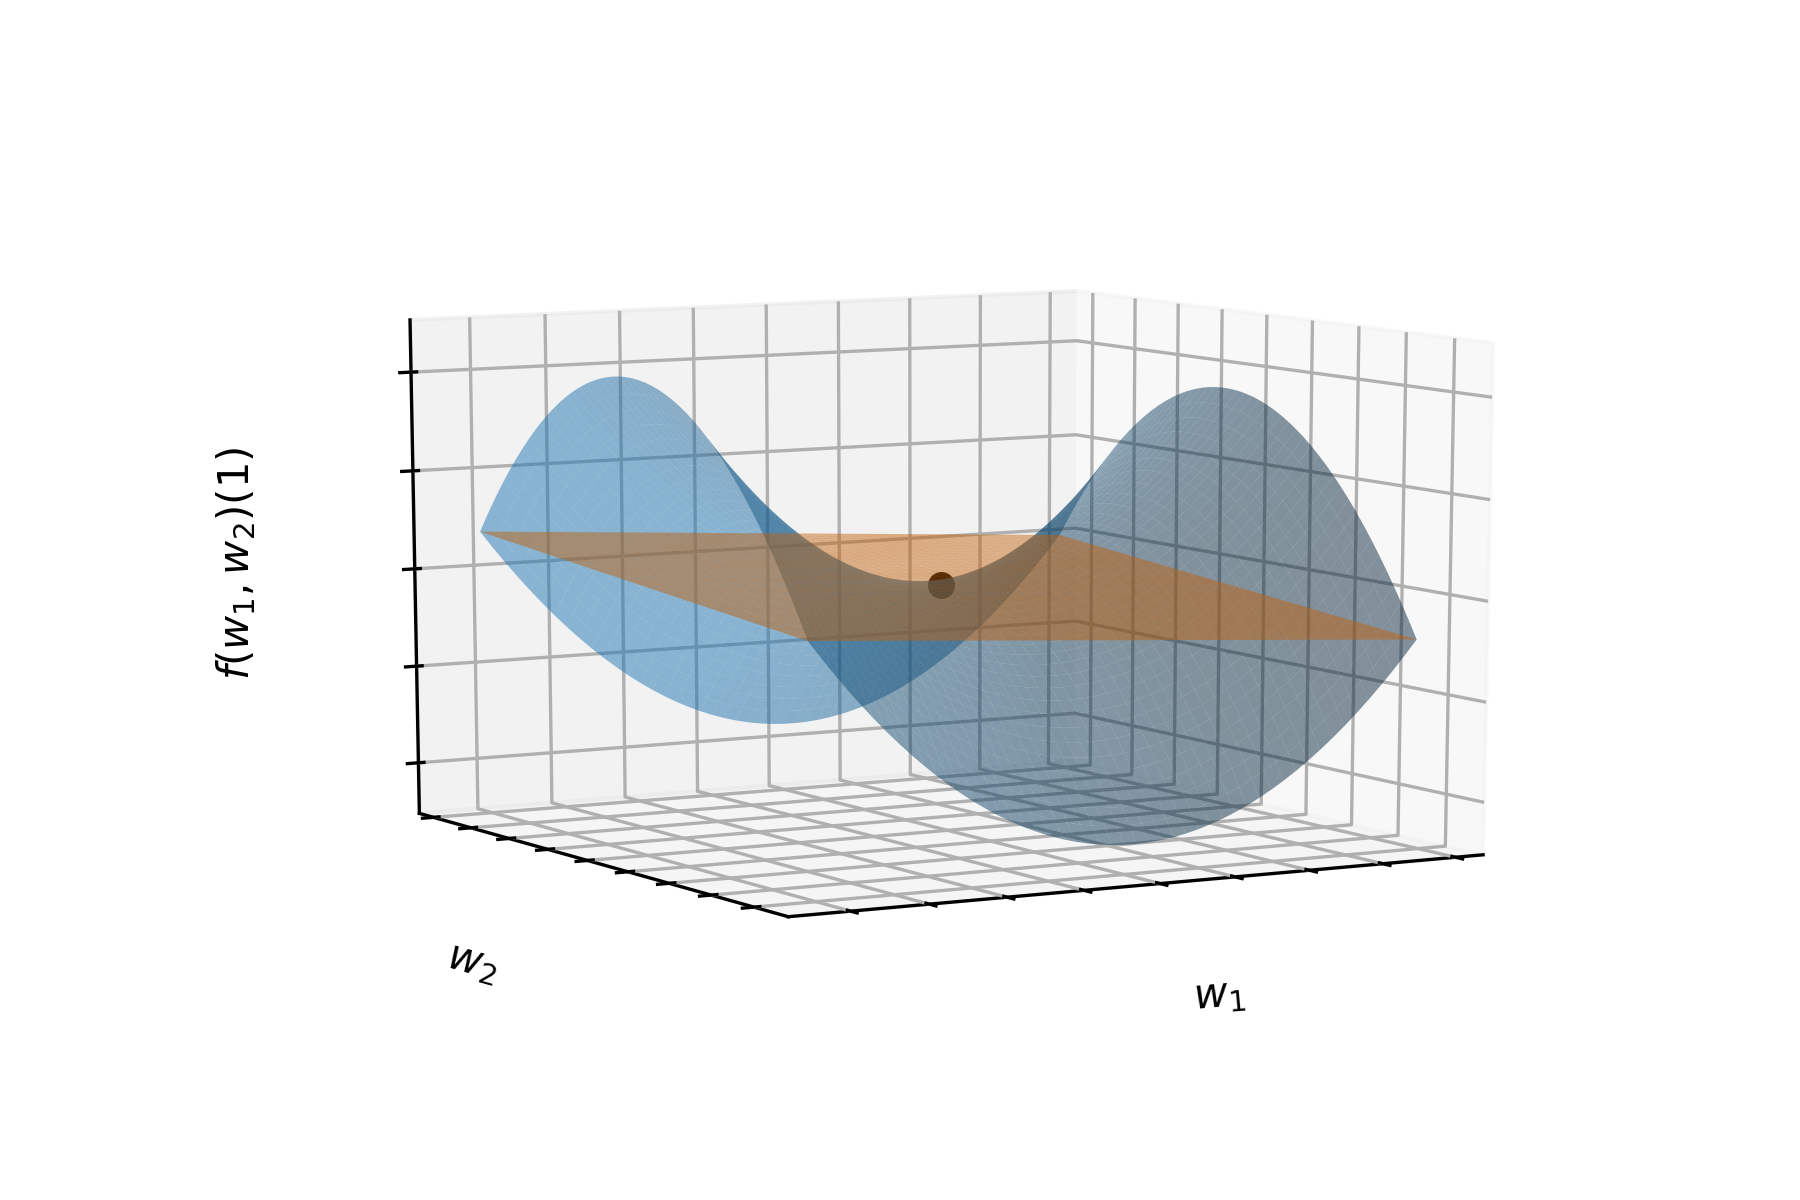
\includegraphics[width=.5\textwidth]{imgs/visualize_linearized_0.1.png}\hfill
    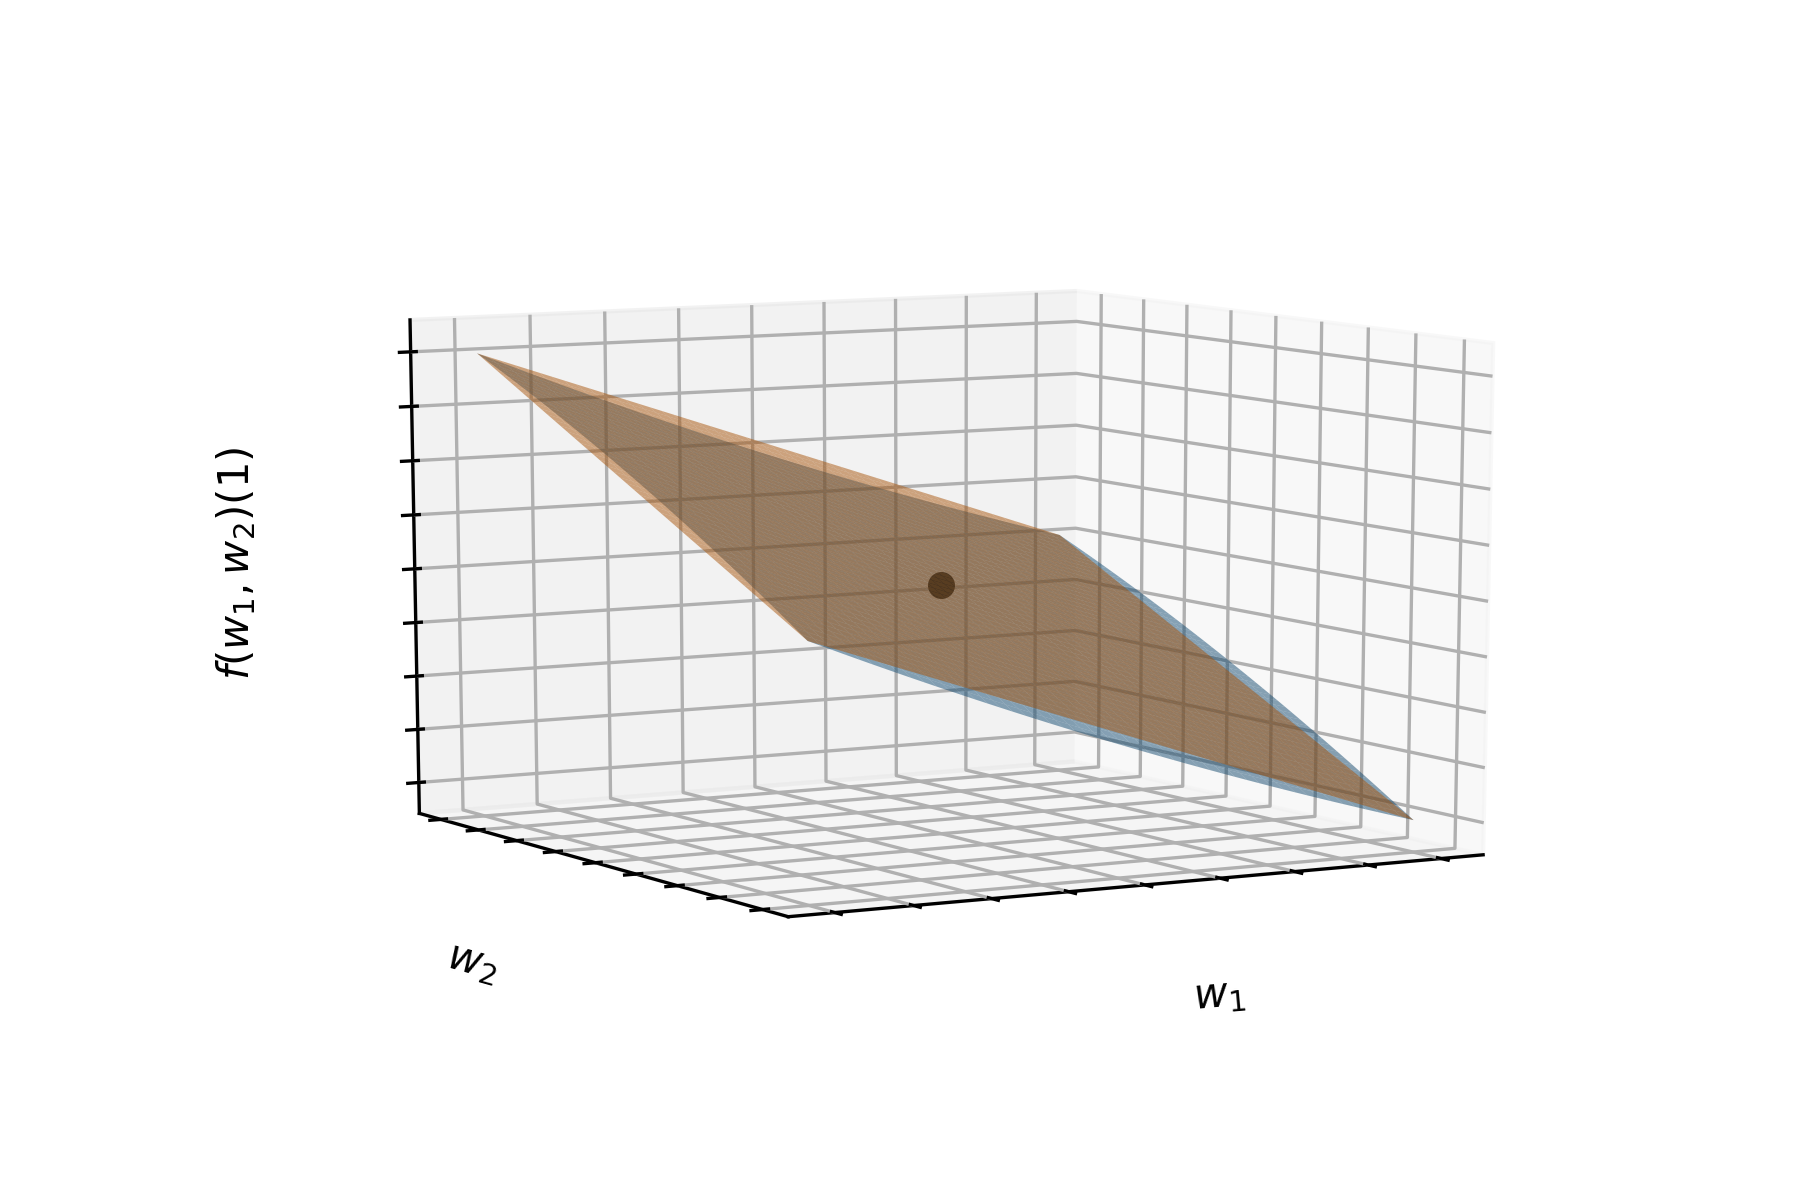
\includegraphics[width=.5\textwidth]{imgs/visualize_linearized_10.png}
    \caption{A neural network with two weights $w_1$, $w_2$ evaluated at the input $1 \in \mathbb{R}$. On the left, notice that the network is highly nonlinear (and nonconvex) in its weights. Conversely, on the right, we see that the function is close to the linearization around its initialization, and so we are approaching the lazy regime.}
\end{figure}

\section{Mathematical Formulation of \enquote{Lazy Training}}

Having provided some intuition for lazy training, we proceed to formalize it mathematically. This formalization will assist us in stating the results we will eventually prove for our project. For the sake of convenience, the notation we use is the same as that presented in \cite{chizat2018lazy}.

In particular, we will consider $\mathbb{R}^p$ the parameter space, $\mathcal{F}$ a Hilbert space, $h: \mathbb{R}^p \rightarrow \mathcal{F}$ a smooth model, and $R: \mathcal{F} \rightarrow \mathbb{R}_+$ a smooth loss function. Notice here that $h$ does not map inputs to outputs, but rather a vector of parameters to a predictor function. Let us use $f(w, \cdot)$ to denote $h(w)$. 

In the case of neural networks, let us take $\rho \in \mathcal{P}(\mathbb{R}^d \times \mathbb{R}^k)$ to be a probability measure on $\mathbb{R}^d \times \mathbb{R}^k$, where $\mathbb{R}^d$ is the input space of the network and $\mathbb{R}^k$ is the output space. We could choose $\mathcal{F} = L^2(\rho_x, \mathbb{R}^k)$, for $\rho_x$ the marginal distribution of the network inputs. This is saying that, for each fixed parameter vector $\mathbb{R}^p$, we get a network function that is square integrable with respect to the distribution of input samples. Furthermore, we could take $\ell: \mathbb{R}^k \times \mathbb{R}^k \rightarrow \mathbb{R}_+$ to be some loss function, and from here define the risk $R(h(w)) = \mathbb{E}_{(X, Y) \sim \rho}\ell(f(w, X), Y)$. If $\rho$ is a finite, discrete probability measure, then $R$ represents the empirical risk (it is simply the loss of each $(x, y)$ weighted by the probability of $(x, y)$); otherwise, $R$ represents the population risk.

With the initialization $w_0 \in \mathbb{R}^p$, we define the linearized model to be 
\begin{align*}
\overline{h}(w) = h(w_0) + Dh(w_0)(w - w_0).
\end{align*}
As we had previously discussed, this is simply the linearization of $h$ around its initialization. Once again, for the particular case of $h$ mapping a parameter vector $w \in \mathbb{R}^p$ to a neural network $f(w, \cdot)$, we get
\begin{align*}
    f(w, x) = f(w_0, x) + Df_w(w_0, x)(w - w_0). 
\end{align*}
In even greater specificity, when the output of the network is one-dimensional, then our linearized model is
\begin{align*}
    f(w, x) = f(w_0, x) + \nabla f_w(w_0, x)(w - w_0). 
\end{align*}

The principal results of \cite{chizat2018lazy} focus on the objective functions $R(h(w))$ and $R(\overline{h}(w))$ when their outputs are scaled by some positive factor $\alpha > 0$:
\begin{align*}
    F_{\alpha}(w) = \frac{1}{\alpha^2}R(\alpha h(w)) \qquad
    \overline{F}_{\alpha}(w) = \frac{1}{\alpha^2}R(\alpha \overline{h}(w)).
\end{align*}
We mention that when the model $h$ is $m$ positively homogeneous, then scaling the model output by $\alpha$ is equivalent to scaling the model weights by $\alpha^{1/m}$. Under suitable conditions on the model $h$ and the loss function $R$, \cite{chizat2018lazy} proves that as $\alpha \rightarrow \infty$, the gradient flow of the objective $F_{\alpha}(w)$, denoted $(w_{\alpha}(t))_{t \geq 0}$, approaches that of the the linearized objective $\overline{F}_{\alpha}(w)$, denoted $(\overline{w}_{\alpha}(t))_{t \geq 0}$. That is to say, for a neural network that is positively homogeneous its weights, by taking the scale with which we initialize the weights to infinity, then training the model with gradient flow is equivalent to gradient flow on the linearized objective.

From here, we see that the implications of lazy training in the contemporary field of deep learning are immediately clear. For instance, lazy training answers the question of what it means when we initialize the weights of our network with large variance. And so we devote our project to studying the proofs of the previously summarized result (that the gradient flow of $F_{\alpha}(w)$ approaches that of $\overline{F}_{\alpha}(w)$) given in \cite{chizat2018lazy}. Interestingly, this is not the only case in which the \enquote{lazy regime} occurs. \cite{jacot2018neural} proves that under suitable conditions on the network, then as its \enquote{width} (number of neurons in its hidden layers) tends to infinity, training the network is equivalent to a kernel method.

\pagebreak 
\section{Theoretical Results}
For each of the results we will prove, we rely on the following set of assumptions:
\begin{assumption}
The model $h: \mathbb{R}^p \rightarrow \mathcal{F}$ is differentiable with a locally Lipschitz differential $Dh$. Note that $D(h): \mathbb{R}^p \rightarrow \mathcal{F}$, by the definition of the derivative, is a continuous linear map. And so the Lipschitz condition on $Dh$ is with respect to the operator norm. Moreover, we assume that the loss function $R$ is differentiable with a Lipschitz gradient.
\end{assumption}

The first result in which I am interested is presented in the appendix of \cite{chizat2018lazy}. This result is of particular relevance to my present research, which deals with the generalization properties of neural networks trained in the lazy regime. In particular, if the gradient flow on the scaled objective function approaches that on the scaled linearized objective, what does this mean about the corresponding models $f(w(t), \cdot)$, $f(\overline{w}(t), \cdot)$? In particular, would we expect $f(w(t), x) \approx f(\overline{w}(t), x)$, even for those $x$ which are not contained in our training set? This question is addressed in the following result:
\begin{manualproposition}{A.1}
Assume for some $C > 0$ it holds that $\Vert w_{\alpha}(T) - \overline{w}_{\alpha}(T) \Vert \leq C\log(\alpha)/\alpha^2$. Assume moreover that there exists a set $\mathcal{X} \subset \mathbb{R}^d$ such that $M_1 := \sup_{x \in \mathcal{X}} \Vert D_wf(w_0, x) \Vert < \infty$ and $M_2 := \sup_{x \in \mathcal{X}} \text{Lip}(w \mapsto Df(w, x)) < \infty$. Then it holds 
\begin{align*}
    \sup_{x \in \mathcal{X}} \Vert \alpha f(w_{\alpha}(T), x) - \alpha \overline{f}(\overline{w}_{\alpha}(T), x) \Vert \leq C \frac{\log(\alpha)}{\alpha}\left(M_1 + \frac{1}{2}C\cdot M_2 \cdot \log(\alpha) \right) \longrightarrow 0 \quad \text{as $\alpha \longrightarrow \infty$}.
\end{align*}
\end{manualproposition}
Notice that the first assumption $\Vert w_{\alpha}(T) - \overline{w}_{\alpha}(T) \Vert \leq C\log(\alpha)/\alpha^2$ is proven in Theorem \ref{finitehorizon}, which we discuss next.

The second result that I wish to prove confirms that lazy training does, in fact, occur in the limit as the scale $\alpha \rightarrow \infty$. However, it is important to mention that this result is weaker than we would like, since it gives bounds on the difference between gradient flow on the original objective and the linearized objective in terms of a finite time horizon $0 \leq t \leq T$.
\begin{manualtheorem}{2.2}\label{finitehorizon}
Assume that $h(w_0) = 0$. Given a fixed time horizon $T > 0$, it holds that $\sup_{t \in [0, T]} \Vert w_{\alpha}(t) - w_0 \Vert = \mathcal{O}(1/\alpha)$,
\begin{align*}
    \sup_{t \in [0, T]} \Vert w_{\alpha}(t) - \overline{w}_{\alpha}(t) \Vert = \mathcal{O}(1/\alpha^2) \quad \text{and} \quad \sup_{t \in [0, T]} \Vert \alpha h(w_{\alpha}(t)) - \alpha \overline{h}(\overline{w}_{\alpha}(t)) \Vert = \mathcal{O}(1/\alpha).
\end{align*}
\end{manualtheorem}

The final, and clearly the most important, result that I will consider gives bounds on the difference between gradient flow on the original and linearized objectives that are uniform in time. Moreover, this result proves that gradient flow on the linearized objective converges exponentially in time to a global minimizer of the loss $R$, denoted $y^{\star} \in \mathcal{F}$. Of course, we will need stronger assumptions on the model $h$ and loss $R$ in order to prove this powerful statement. 
\begin{manualtheorem}{2.4}\label{uniformbound}
Consider the $M$-smooth and $m$-strongly convex loss $R$ with minimizer $y^{\star}$ and condition number $\kappa := M/m$. Assume that $\sigma_{\text{min}}$, the smallest singular value of $Dh(w_0)^T$, is positive and that the initialization satisfies $\left\Vert h(w_0) \right\Vert \leq C_0:= \sigma_{\text{min}}^3/(32\kappa^{3/2} \left\Vert Dh(w_0) \right\Vert \text{Lip}(Dh))$, where $\text{Lip}(Dh)$ is the Lipschitz constant of $Dh$. If $\alpha > \left\Vert y^{\star} \right\Vert / C_0$, then for $t \geq 0$, it holds
\begin{align*}
    \left\Vert \alpha h(w_{\alpha}(t)) - y^{\star} \right\Vert \leq \sqrt{\kappa} \left\Vert \alpha h(w_0) - y^{\star} \right\Vert \exp( -m \sigma_{\text{min}}^2 t/4).
\end{align*}
If moreover $h(w_0) = 0$, it holds as $\alpha \rightarrow \infty$, $\sup_{t \geq 0} \left\Vert w_{\alpha}(t) - w_0 \right\Vert = \mathcal{O}(1/\alpha)$,
\begin{align*}
    \sup_{t \geq 0} \left\Vert \alpha h(w_{\alpha}(t)) - \alpha \overline{h}(\overline{w}_{\alpha}(t)) \right\Vert = \mathcal{O}(1/\alpha) \quad \text{and} \quad  \sup_{t \geq 0} \left\Vert w_{\alpha}(t) - \overline{w}_{\alpha}(t) \right\Vert = \mathcal{O}(\log \alpha/\alpha^2).
\end{align*}
\end{manualtheorem}

Admittedly, the proof of Theorem \ref{uniformbound} given by \cite{chizat2018lazy} is quite technical and challenging, and so understanding even a portion of the authors' argument would be a rewarding endeavor. While I would like to understand the entirety of their argument, I might need to settle for studying only a portion of the result.


\pagebreak
\bibliographystyle{siam}
\bibliography{biblio}

\end{document}